\begin{figure}
  \setlength{\unitlength}{\textwidth}

        \begin{picture}(1,0.4)(0,0.4)

      \put(0.1,0.45){\includegraphics[width=0.75\unitlength]{../FnP/gnuplot/error.eps}}
      
%       \put(0.07,0.95){$\displaystyle\frac{V}{D}$}
%       \put(0.07,1.3){$\displaystyle\frac{A}{D}$}
       \put(0.05,0.58){\rotatebox{90}{$\% \ error$}}
%       \put(0.5,0.4){$\massdamp$}
       \put(0.5,0.4){\JL{$\massstiff$}}
    \end{picture}

  % \caption{Comparison of maximum power between QSS and DNS data obtained using 3 point local quadratic curve fitting.The error was obtained using Eq:\ref{eqn:error_calculation}}
    \caption{\JL{The difference between the maximum power predicted by
        the QSS model for $\massstiff = 10$, and the DNS data as a
        function of \massstiff. The QSS model prediction is worst for
        low values of \massstiff.}}
    \label{fig:error}
\end{figure}

 %vspace{10cm}
